\section{Overview}
The main high-level components of the system that will be taken into account are structured in four layers, as shown in Figure \ref{img:layeredStructure} below.

\begin{figure}[H]
  \begin{center}
  	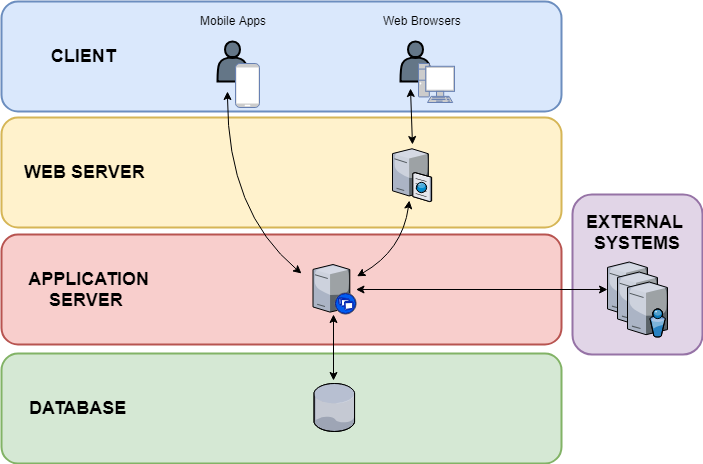
\includegraphics[width=\textwidth]{./img/LayeredStructure.png}
    \hspace{0.05\linewidth}
    \centering
    \caption{\textit{Layered Structure} of the system.}
		\label{img:layeredStructure}
    \end{center}
\end{figure}

The considered high-level components are:
\begin{itemize}
  \setlength{\itemindent}{-.4in}
  \item[] \textbf{Mobile Applications:} The \textit{Presentation Layer} dedicated to mobile devices; it communicates with the Application Server.
  \item[] \textbf{Web Browsers:} The \textit{Presentation Layer} dedicated to web browsers; it communicates directly with the Web Server.
  \item[] \textbf{Web Server:} This is the layer that provides web-pages for the web-based applications; it communicates with the Application Server and with the Web Browsers.
  \item[] \textbf{Application Server:} This is the layer in which is contained all the \textit{logic} for the application; it communicates with the Web Server and with the Database. Moreover it manages the communication with External Services.
  \item[] \textbf{Database:}  The \textit{Data Layer} of the system; it includes all structures and entities responsible for data storage and management. It communicates with the Application Server.
\end{itemize}
It has been taken the decision to separate the Application and Web Server in order to allow greater scalability. In the figure above it is also shown the interaction between the Application Server and External Systems.
A more detailed description of the intereactions between the described system components is shown in Figure \ref{img:highLevelComponents}.

\begin{figure}[H]
  \begin{center}
  	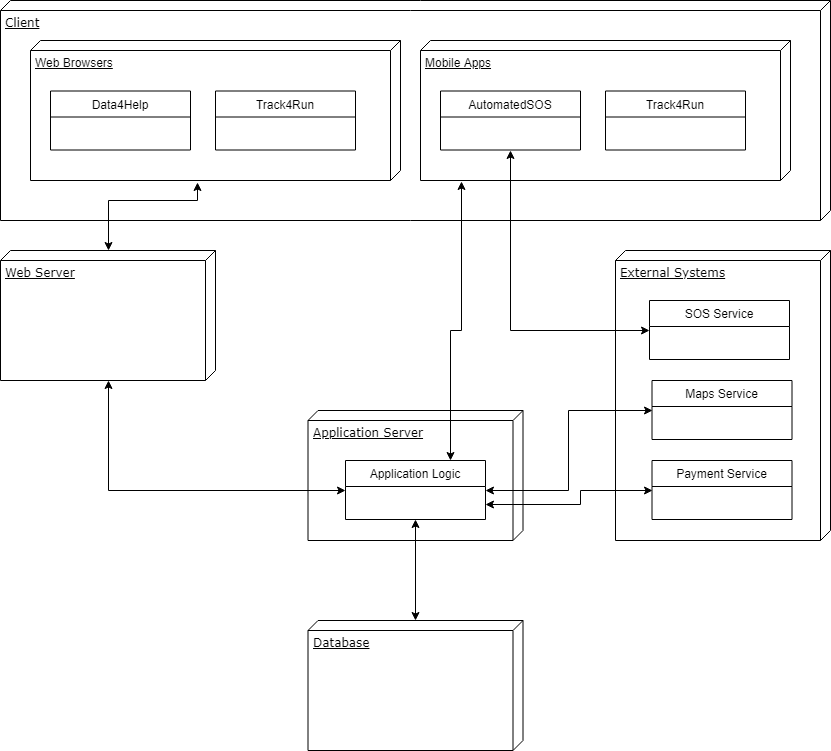
\includegraphics[width=\textwidth]{./img/HighLevelComponents.png}
    \hspace{0.05\linewidth}
    \centering
    \caption{\textit{High Level Components} of the system.}
		\label{img:highLevelComponents}
    \end{center}
\end{figure}
\section{Component View}
% -- TODO --

\subsection{Database}
The application database will be managed using a Relational DBMS.
It allows the reading of data, ensuring users the ability to log in and access the applications of interest and check the stored data.
It is also used for data manipulation (insertion, modification and deletion).
The use of a Relational DBMS guarantees the fundamental properties for a database of this type:
\begin{itemize}
  \item \textit{Atomicity}: no partial executions of operations.
  \item \textit{Consistency}: the database is always in a consistent state.
  \item \textit{Isolation}: each transaction is executed in an isolated and independent way.
  \item \textit{Durability / Persistence}: changes made are not lost.
\end{itemize}
The database will offer to the Application Server an interface that it can use to interact with the database.
The data stored in the database must be considered personal and confidential, therefore, procedures must be implemented to safeguard the stored information.\\
Particular attention must be paid to the reading permissions granted to users and to the encryption of passwords used to access the services offered.
Below is the designed E-R diagram.(Figure \ref{img:ER_Diagram})

\begin{figure}[H]
  \begin{center}
  	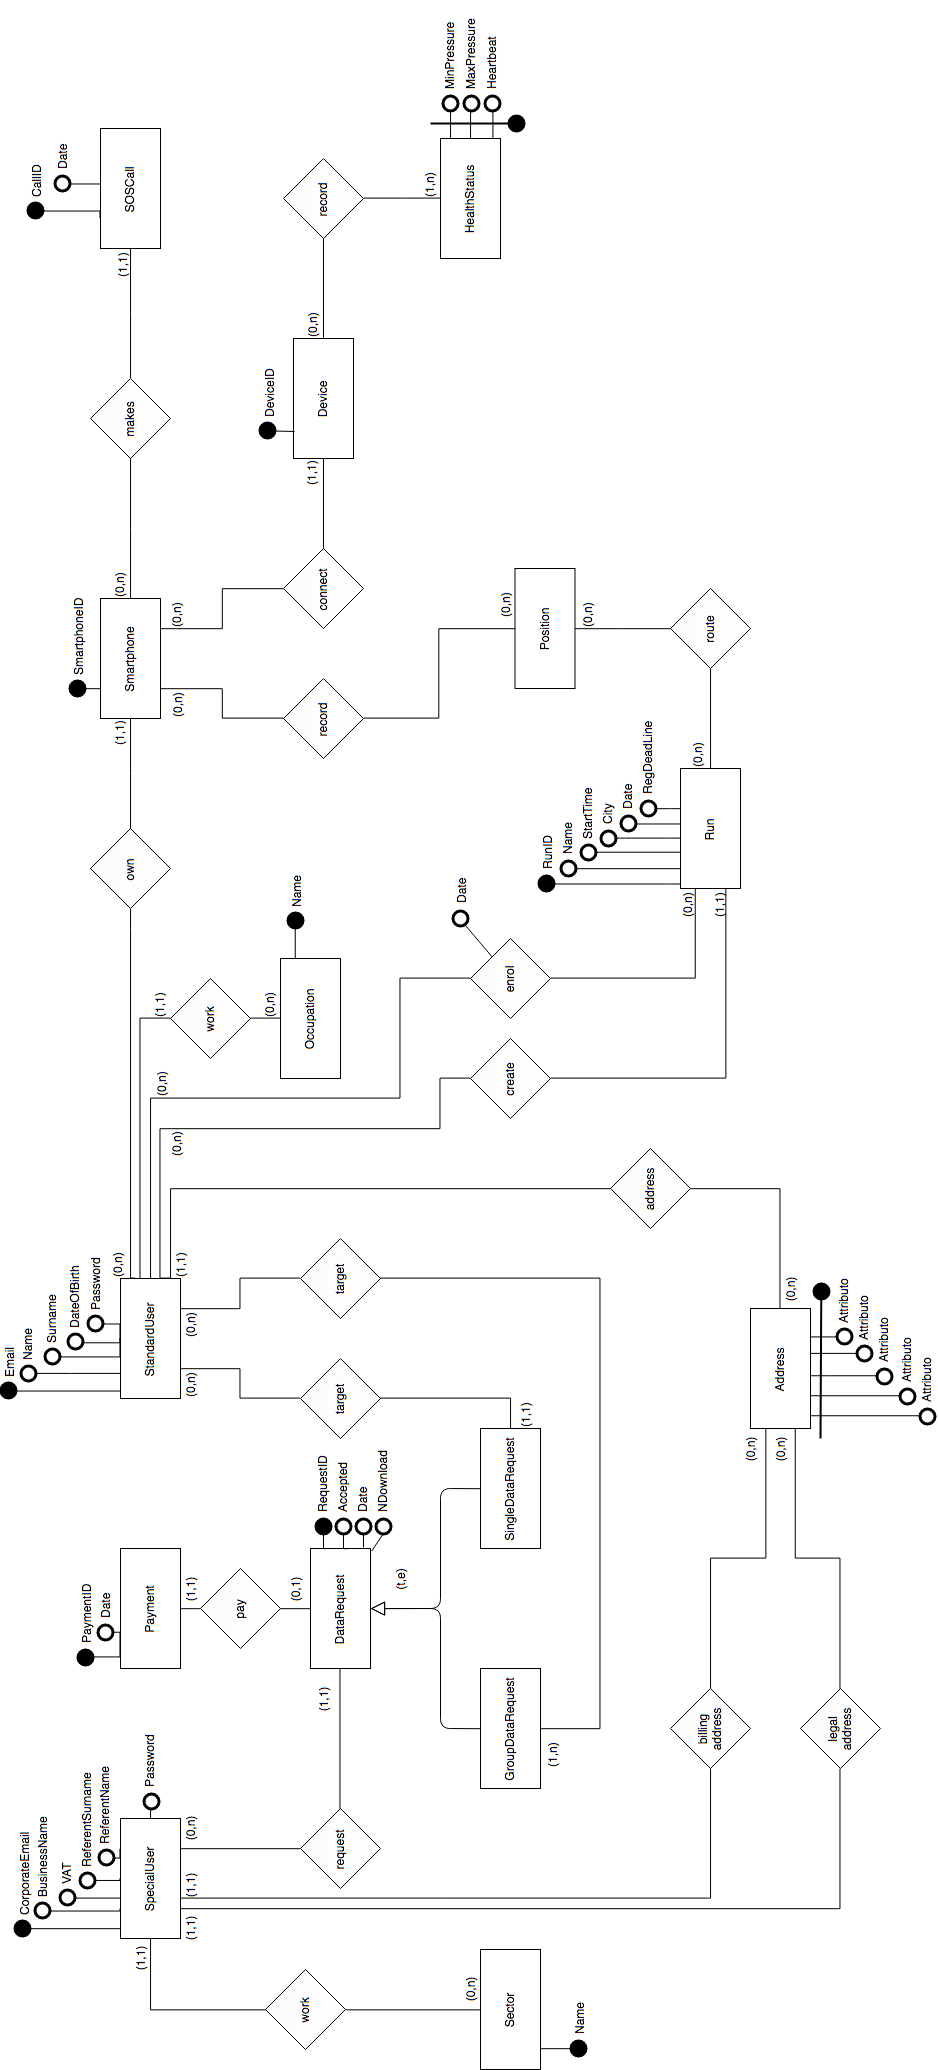
\includegraphics[height=0.68\paperheight]{./img/ER.png}
    \hspace{0.05\linewidth}
    \centering
    \caption{\textit{E-R} Diagram}
		\label{img:ER_Diagram}
    \end{center}
\end{figure}

\subsection{Application Server}
This is the crucial layer of the system to be. The main feature of the \textit{Application Server} is to describe rules and work-flows of all the functionalities provided by the application.\\
The \textit{Application Server} must have intefaces to communicate with the \textit{Web Server} and the \textit{Mobile Apps}, it has also to communicate through interfaces with all the \textit{External Services} (Maps Service, SOS Service and Payment Service).\\
Moreover, the \textit{Application Server} is the only entity of the system that is granted to communicate with the DBMS.
Following this brief introduction there are the logic modules and their descriptions, moreover all connections among components could be seen in the \textit{Global Component View} in Figure \ref{img:GlobalComponent}.

\paragraph{Data Collector Service}
This module offers the a service to the \textit{Standard User Manager} in order to maange user's data and store it into the \textit{Data4Help} database. Data storage is done through \textit{Stored Data Manager}.

\paragraph{Group Request Manager}
This module manages the third party requests of \textit{Group Data Requirement}.

\paragraph{Mail Manager}
This module is a tool for other modules that allow the system to send e-mail, for instance in the registration and enrolment phase.

\paragraph{Maps Manager}
This module is an handler providing an interface to the external service of maps.

\paragraph{Payment Handler}
This module is an handler providing an interface to the external service of payment.

\paragraph{Persistence Unit}
This module is the unique interface to the database's DBMS.

\paragraph{Run Manager}
This module manages \textit{Runs} in all their functionalities, like creation, deletion and enrolment.\\
In order to manage guest users that visit a Run the system this module provides an access point to the \textit{Application Server} for the \textit{Web Server} and the \textit{Mobile Apps}.

\paragraph{Single Request Manager}
This module manages the third party requests of \textit{Single Data Requirement}.

\paragraph{Special User Manager}
This module provides all functionalities related to the \textit{Special User}.

\paragraph{Standard User Manager}
This module provides all functionalities related to the \textit{Standard User}.

\paragraph{Stored Data Manager}
This module provides data to \textit{Group Request Manage} and \textit{Single Request Manage}. It has also to manage all privacy checks and provide data without any type of personal information of the users for \textit{Group Data Requirement}.

\paragraph{User Access Point}
This module provides an access point to the \textit{Application Server} for the \textit{Web Server} and the \textit{Mobile Apps}.
It routes different users in the correct \textit{User Manger} module: Special User and Standard User.



\subsection{Mobile App}
The \textit{Mobile App} must communicate to the \textit{Application Server} through APIs that have to be defined in order to describe the interactions between the two layers and they must be indipendent from the implementation both side.\\
The App UI must be designed user friendly and it has to follow the guidelines provided by the Android and iOS producer.
The application must provide a software module that manages the GPS connection of the device and keeps track of locations data, it has also to manage the Health data from the devices connected to the phone.\\
The application must provide all collected data to the \textit{Application Server} in order to process them.

\subsection{AutomatedSOS App}
In this Section we want to specify in detail the modules that compose the \textit{AutomatedSOS} application in order to better explain the important activity of detection of possible \textit{Critical Situation}.\\
All connections among components could be seen in the \textit{AutomatedSOS Component View} in Figure \ref{img:AutomatedComponent}.

\paragraph{Application Server Handler}
This module is an handler providing an interface to the \textit{Application Server}.

\paragraph{Background Health Monitor}
This module checks status of health data that it receives. If an SOS call must be done it call \textit{SOS Handler}.

\paragraph{GUI}
This module is the \textit{Graphical} interface to the smartphone.

\paragraph{Health Status Service}
This module manage data detected and produce statistic for the \textit{User}.

\paragraph{SOS Handler}
This module is an handler providing an interface to the external service of SOS.

\subsection{Web Server}
The \textit{Web Server} must communicate to the \textit{Application Server} through HTTPS protocol.\\
The \textit{GUI} of the \textit{}{Web Server} must be designed user friendly and it has to follow the guidelines provided by W3C standard (using HTML5, CSS and JS).\\
The \textit{Control Unit} manages all actions played by a user and it must communicate to the \textit{Application Server} through APIs, that are already explained for the \textit{Mobile App}.

\begin{figure}[H]
  \begin{center}
  	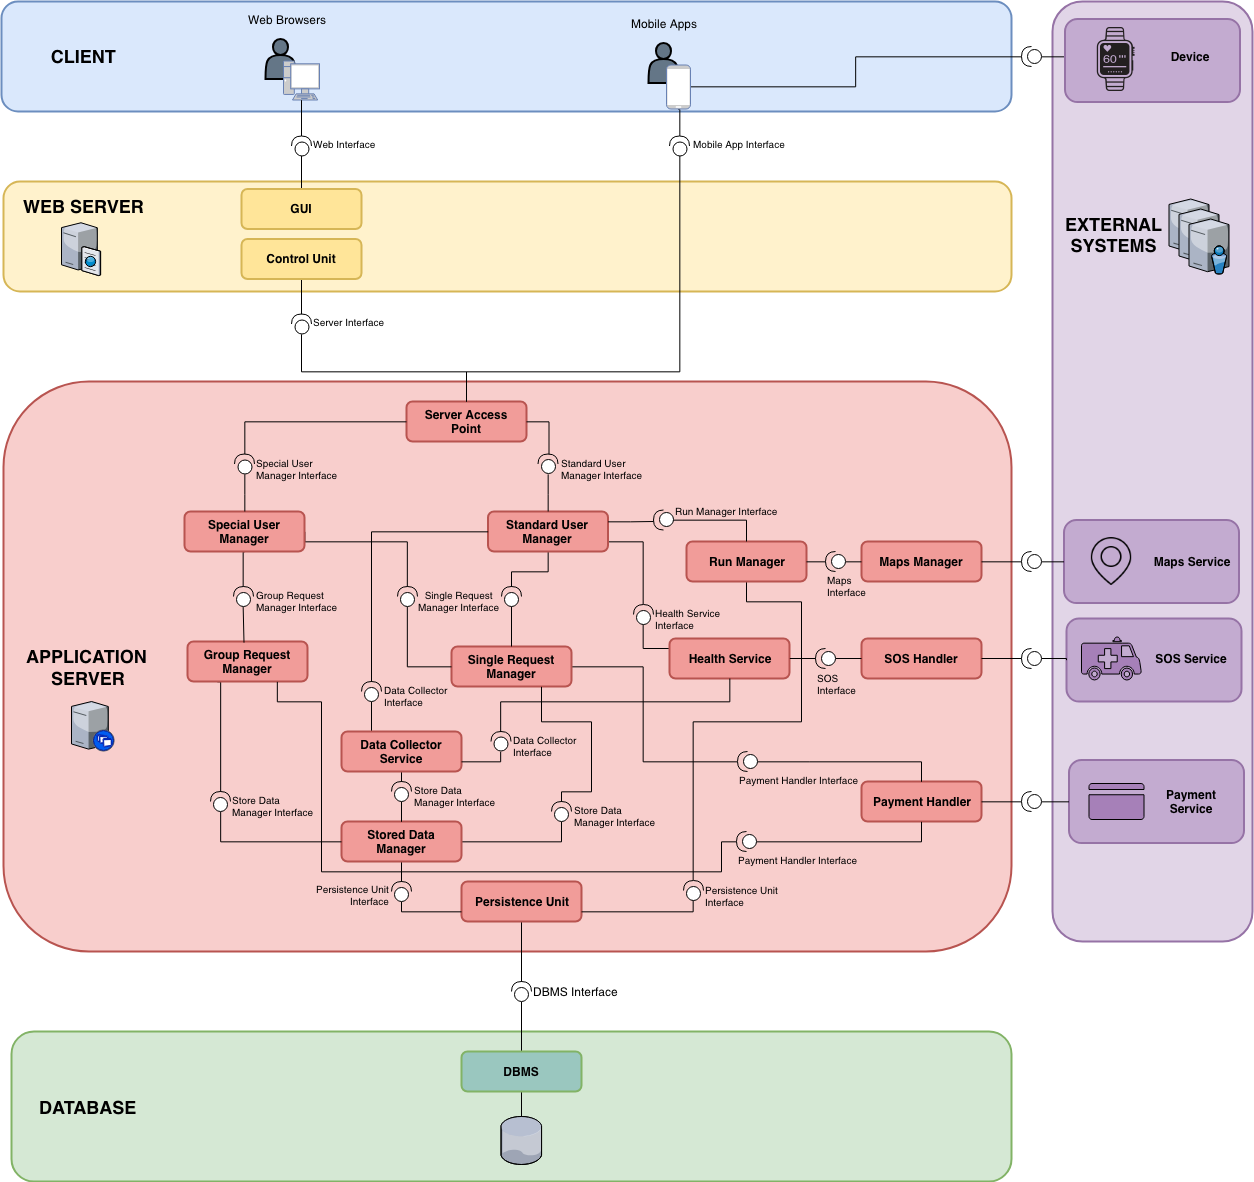
\includegraphics[width=\textwidth]{./img/GlobalComponent.png}
    \hspace{0.05\linewidth}
    \centering
    \caption{\textit{Global Component View}}
		\label{img:GlobalComponent}
    \end{center}
\end{figure}

\begin{figure}[H]
  \begin{center}
  	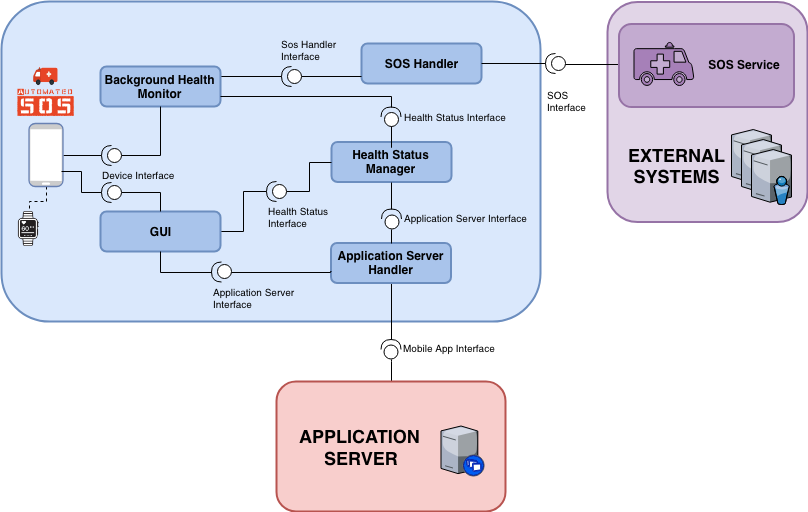
\includegraphics[width=\textwidth]{./img/Automated_Component.png}
    \hspace{0.05\linewidth}
    \centering
    \caption{\textit{AutomatedSOS Component View}}
		\label{img:AutomatedComponent}
    \end{center}
\end{figure}

\section{Deployment View}
Below is the deployment diagram of the system to be (Figure \ref{img:Deployment_Diagram}).

\begin{figure}[H]
  \begin{center}
  	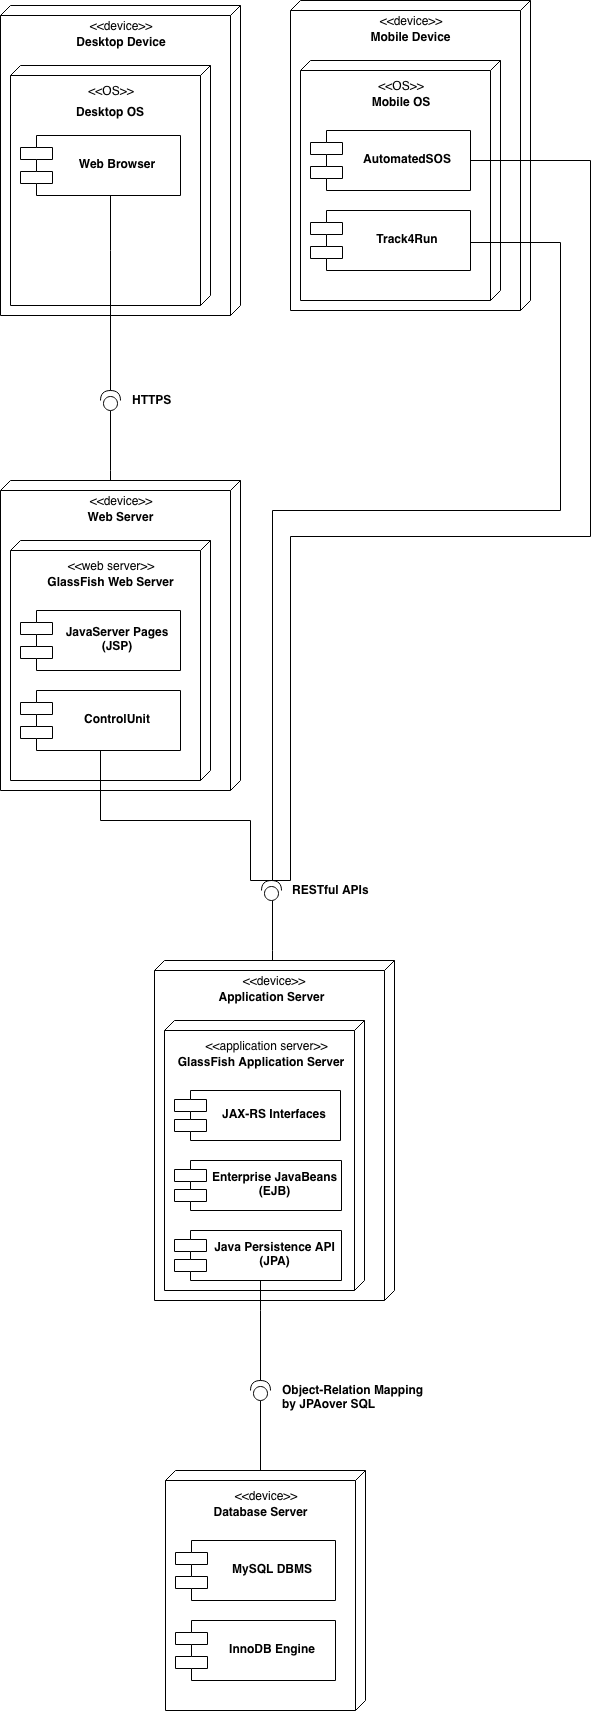
\includegraphics[height=0.68\paperheight]{./img/Deployment_Diagram.png}
    \hspace{0.05\linewidth}
    \centering
    \caption{Deployment Diagram of the system to be}
		\label{img:Deployment_Diagram}
    \end{center}
\end{figure}

\section{Runtime View}
In this Section we want to specify the behaviour of our system. Some relevant cases are selected and explained using Sequence Diagrams.

\begin{figure}[H]
  \begin{center}
  	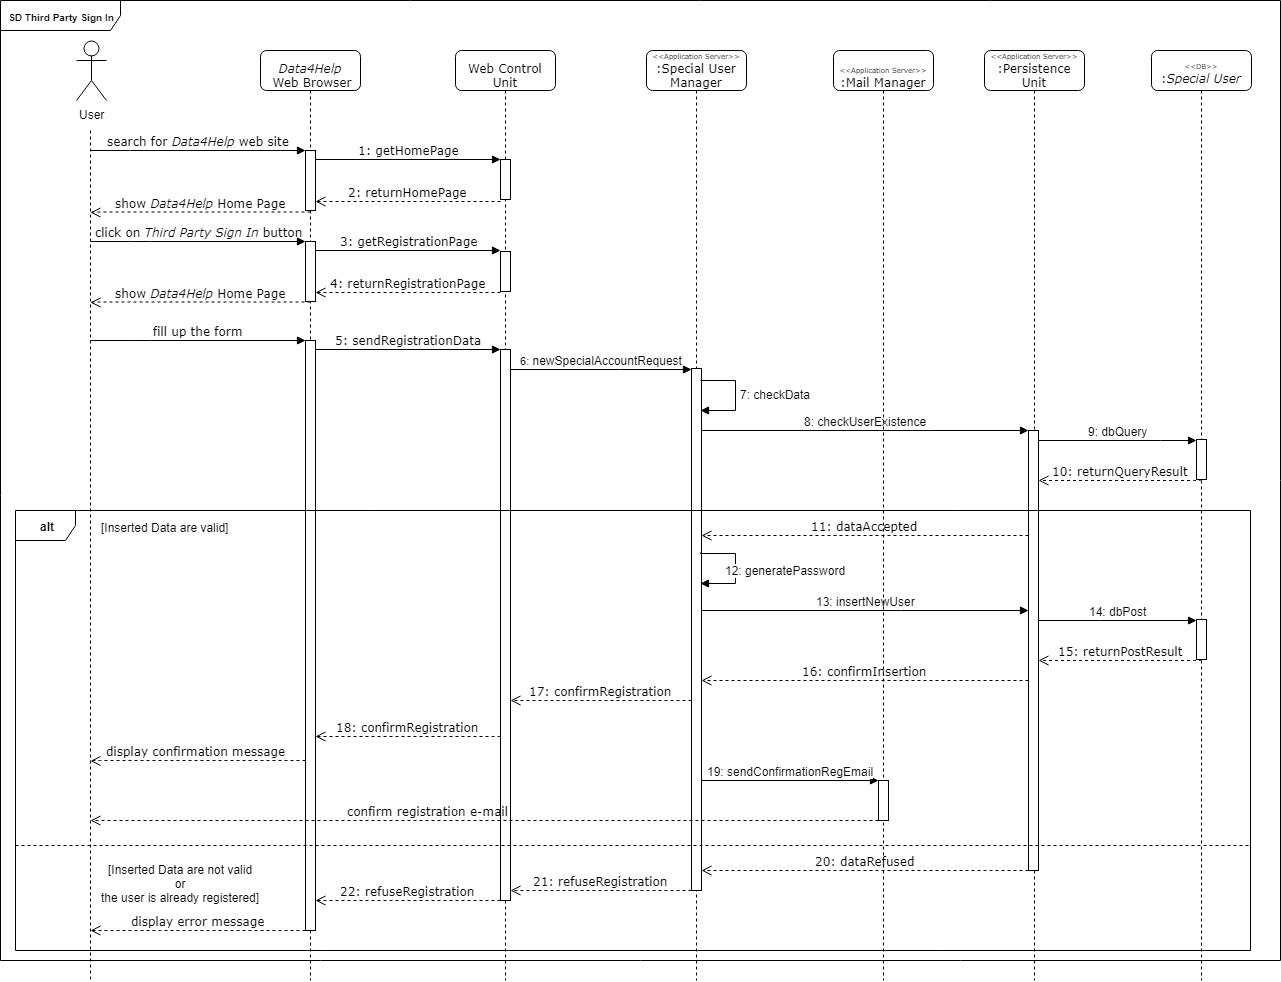
\includegraphics[width=\textwidth]{./img/sequence/webSignIn.png}
    \hspace{0.05\linewidth}
    \centering
    \caption{\textit{Third Party Sign In} sequence diagram}
		\label{img:webSignIn}
    \end{center}
\end{figure}

\begin{figure}[H]
  \begin{center}
  	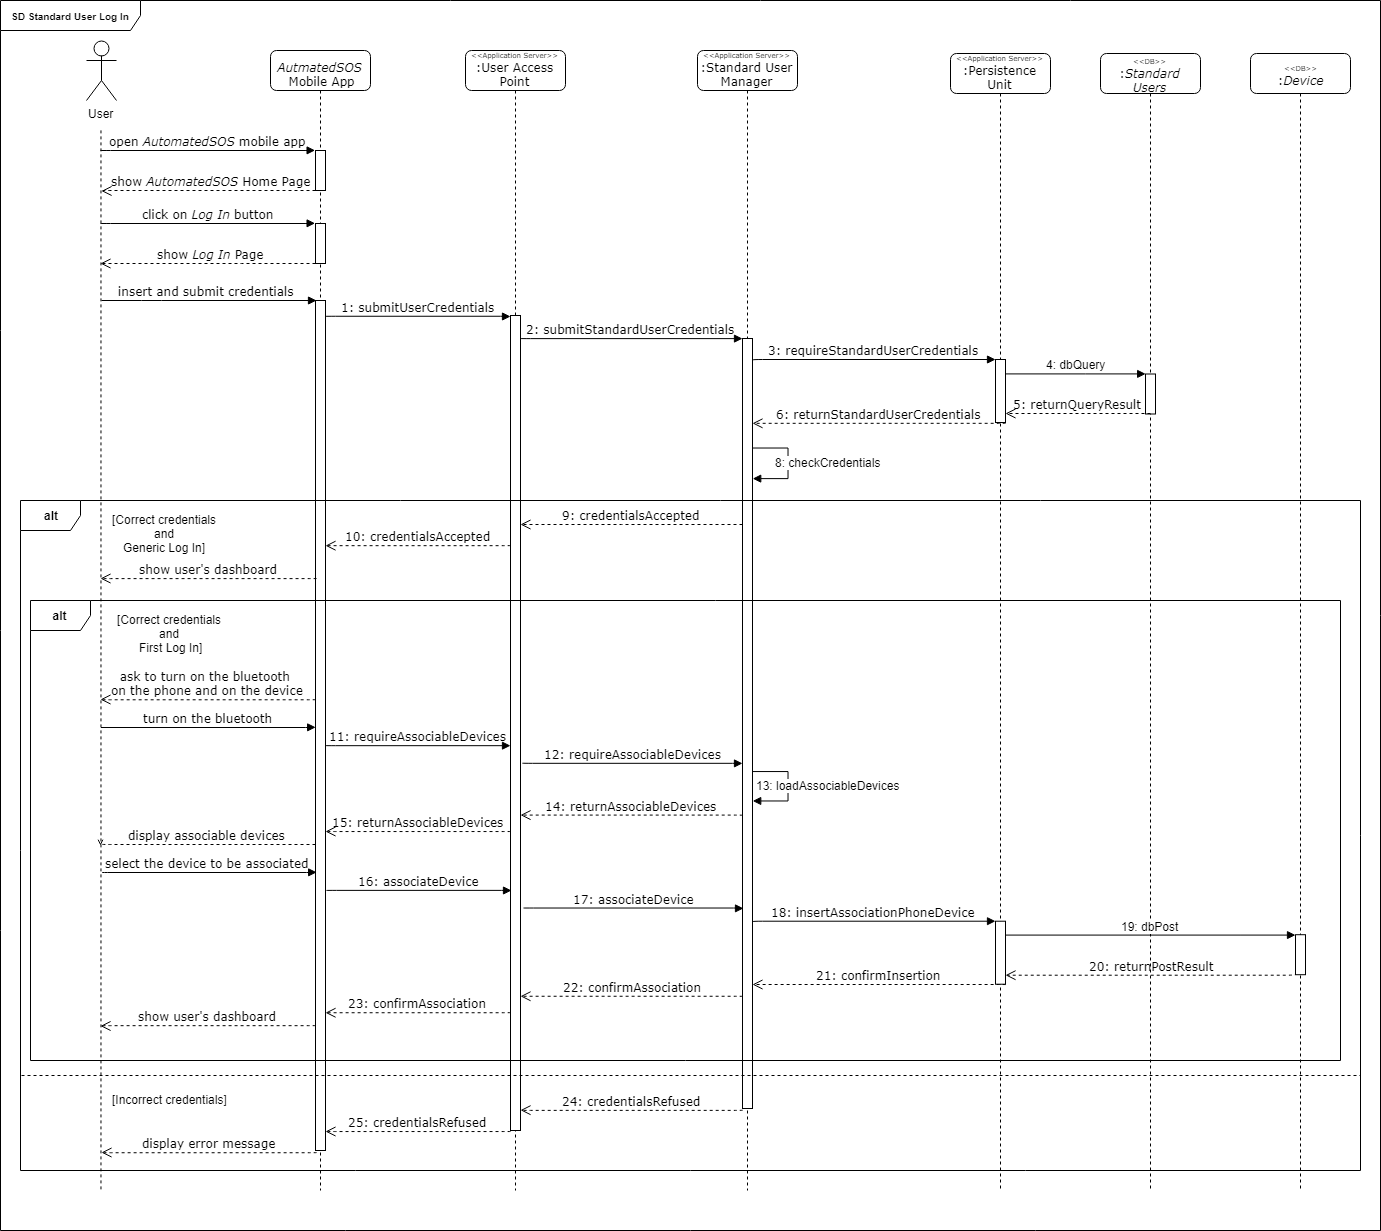
\includegraphics[width=\textwidth]{./img/sequence/appLogIn.png}
    \hspace{0.05\linewidth}
    \centering
    \caption{\textit{Standard User Log In} sequence diagram}
		\label{img:appLogIn}
    \end{center}
\end{figure}

\begin{figure}[H]
  \begin{center}
  	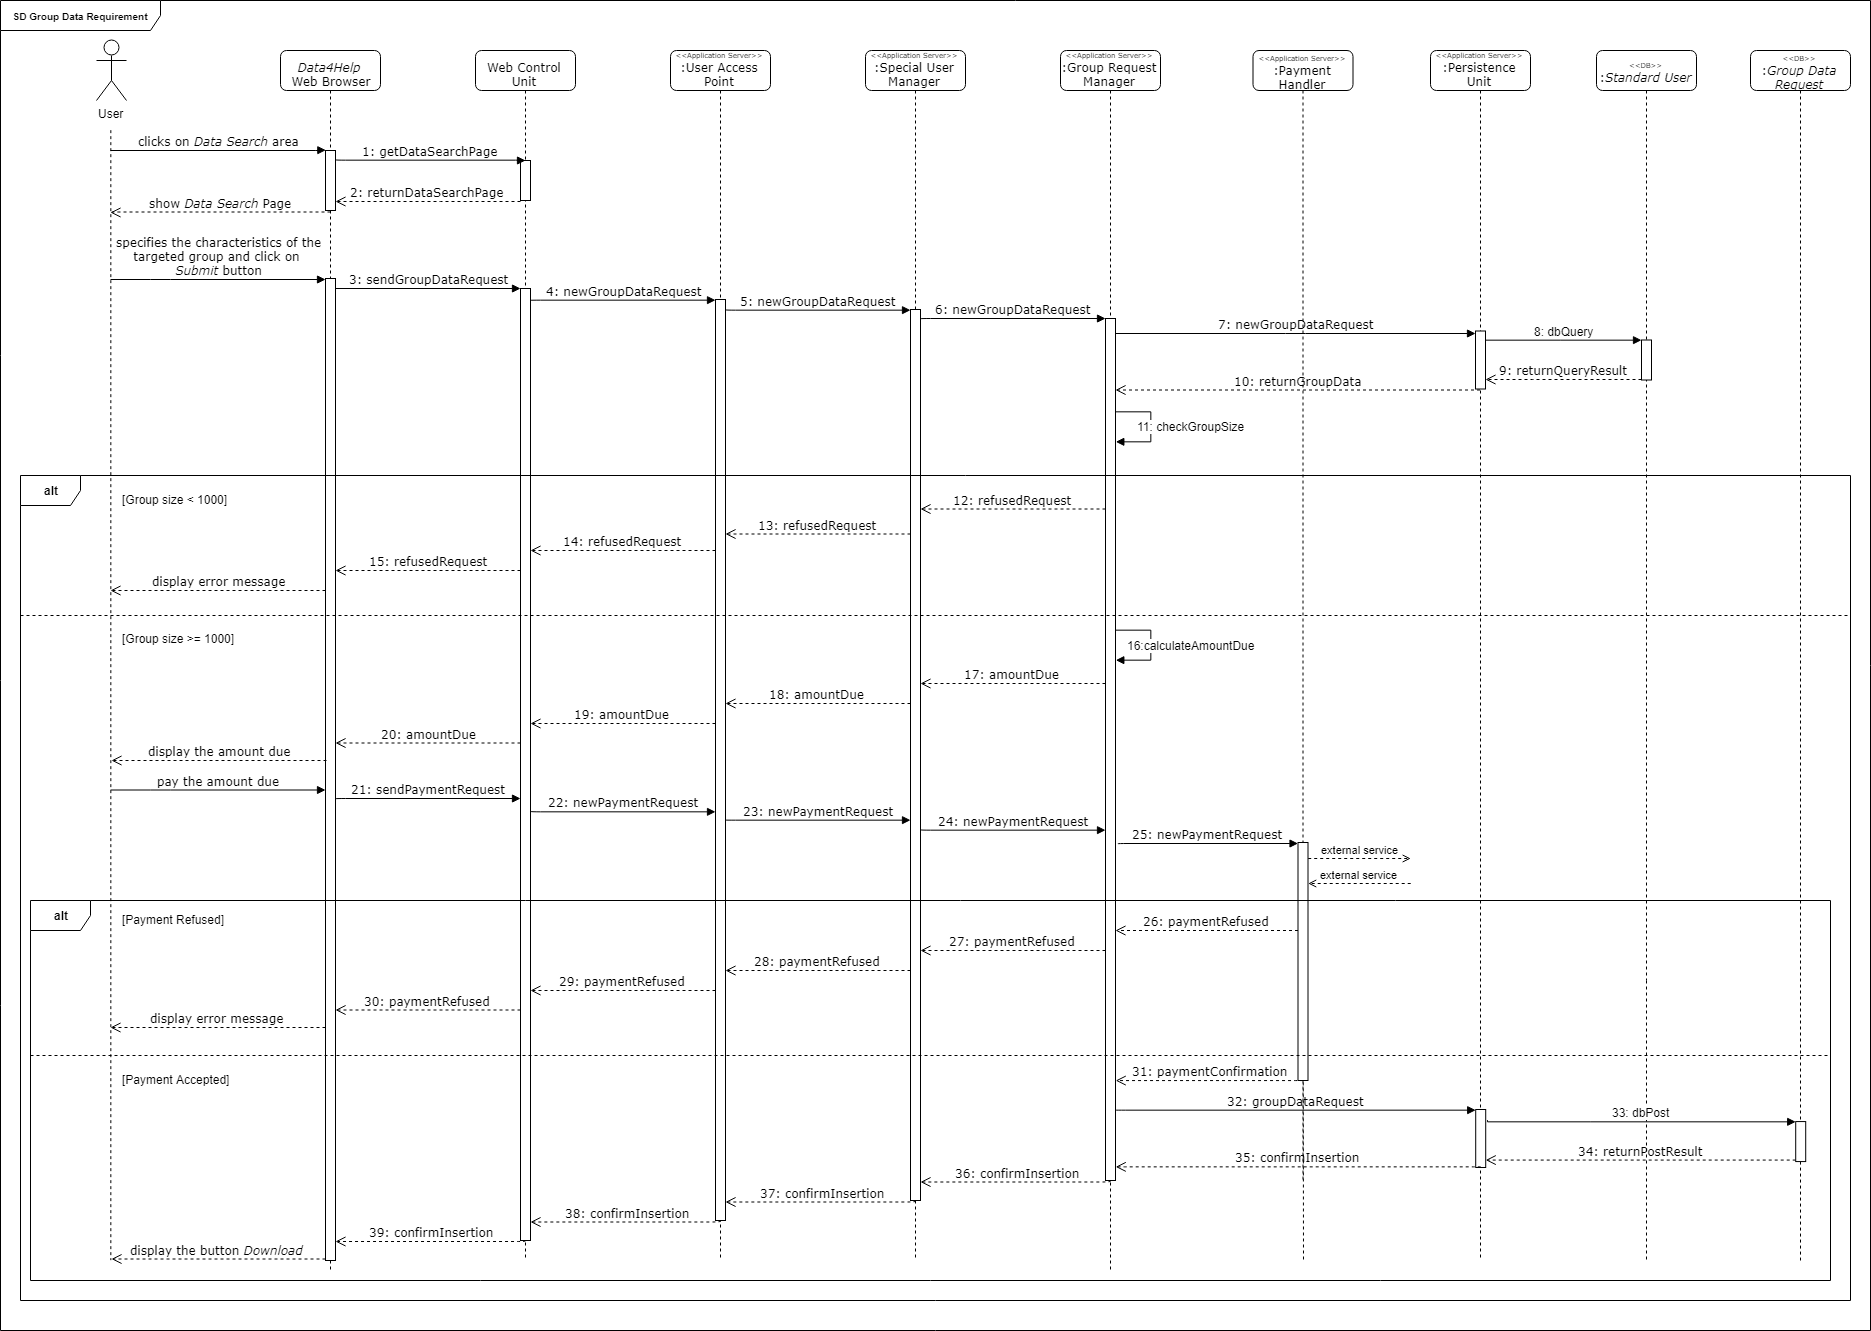
\includegraphics[width=\textwidth]{./img/sequence/groupDataRequest.png}
    \hspace{0.05\linewidth}
    \centering
    \caption{\textit{Group Data Request} sequence diagram}
		\label{img:groupDataRequest}
    \end{center}
\end{figure}

\begin{figure}[H]
  \begin{center}
  	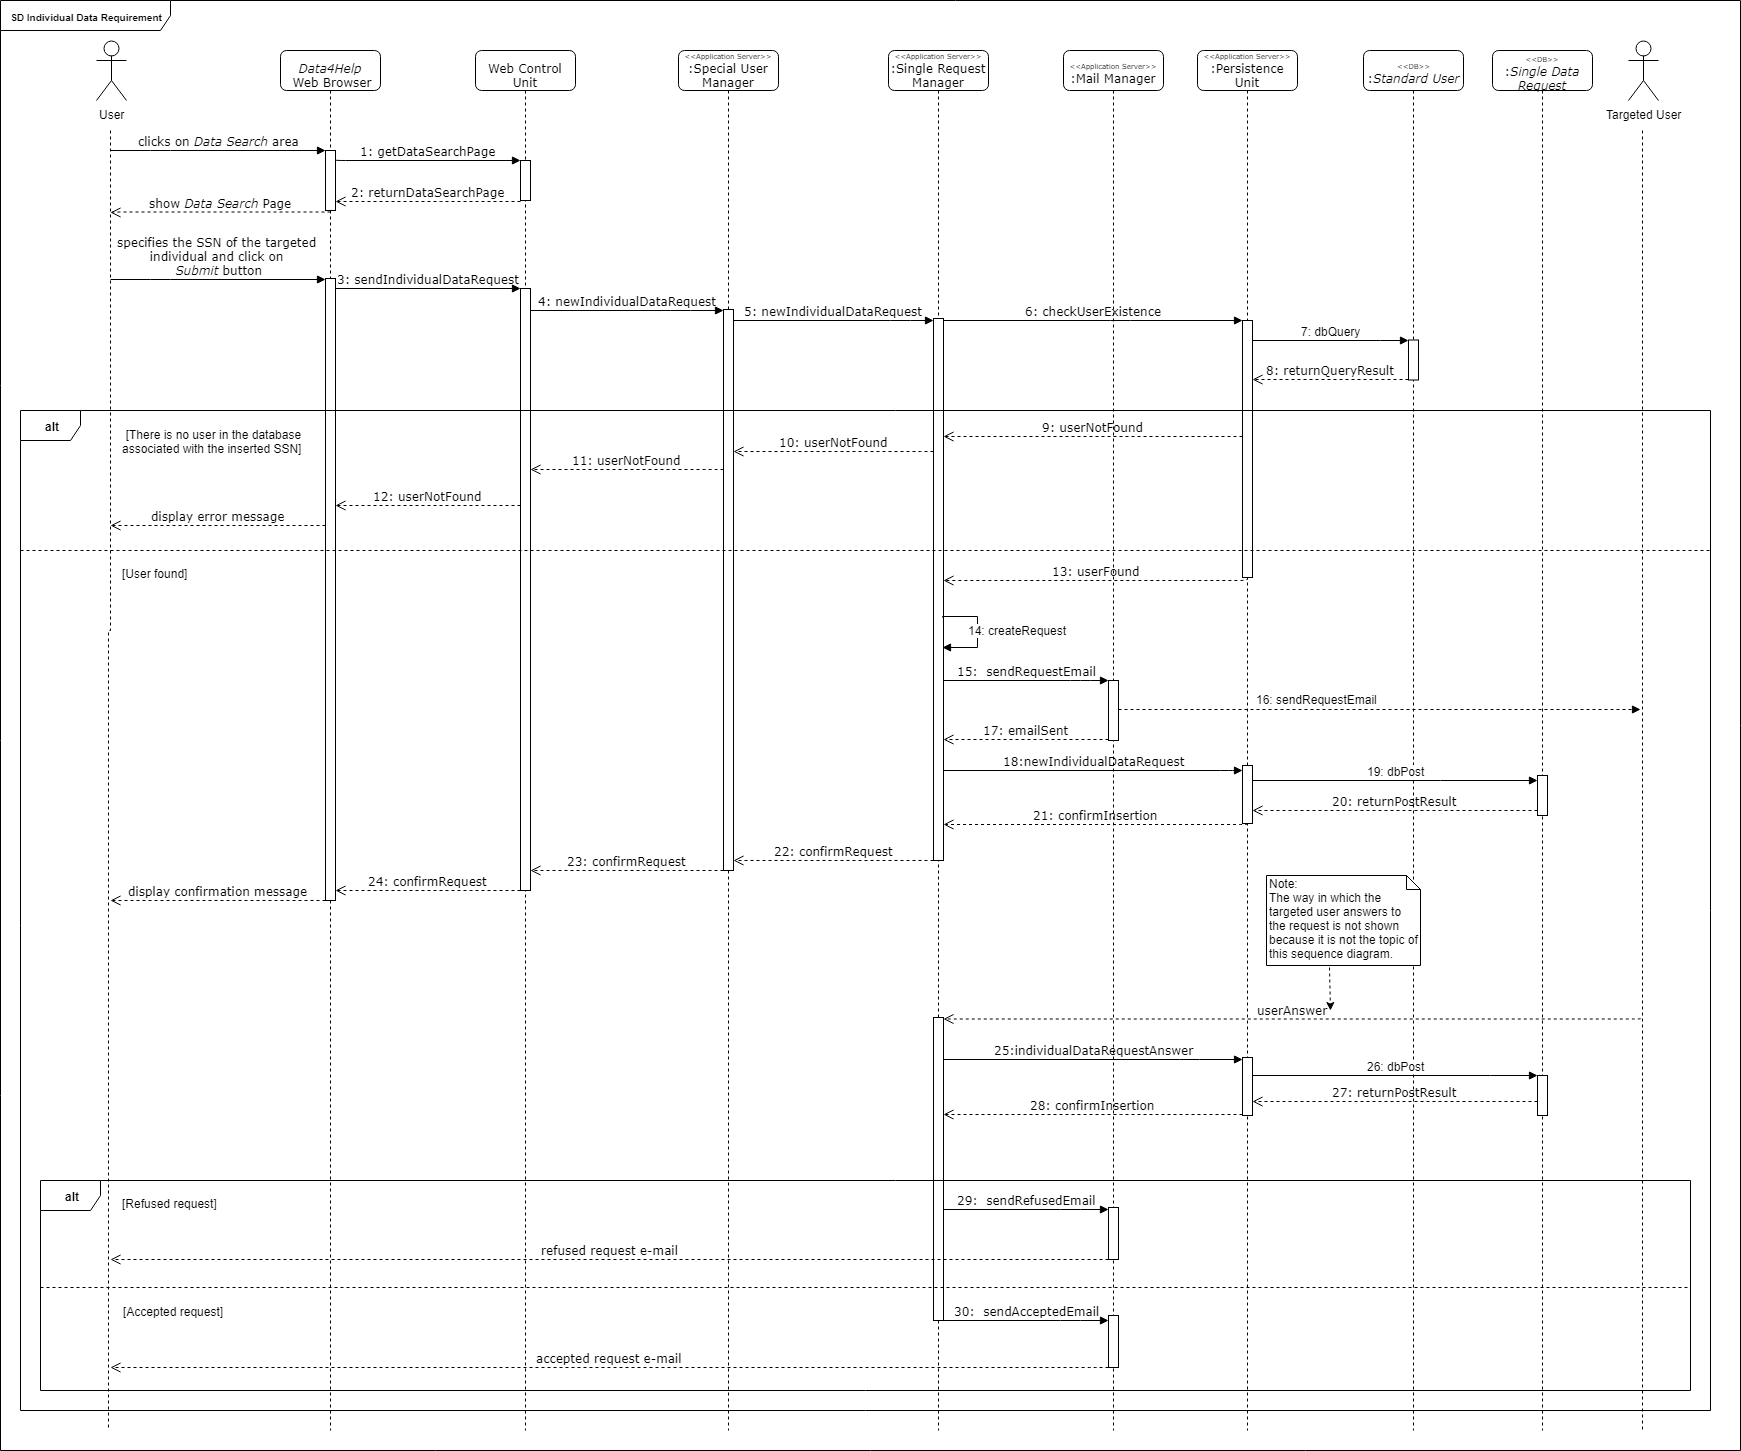
\includegraphics[width=\textwidth]{./img/sequence/individualDataRequest.png}
    \hspace{0.05\linewidth}
    \centering
    \caption{\textit{Individual Data Request} sequence diagram}
		\label{img:individualDataRequest}
    \end{center}
\end{figure}

\begin{figure}[H]
  \begin{center}
  	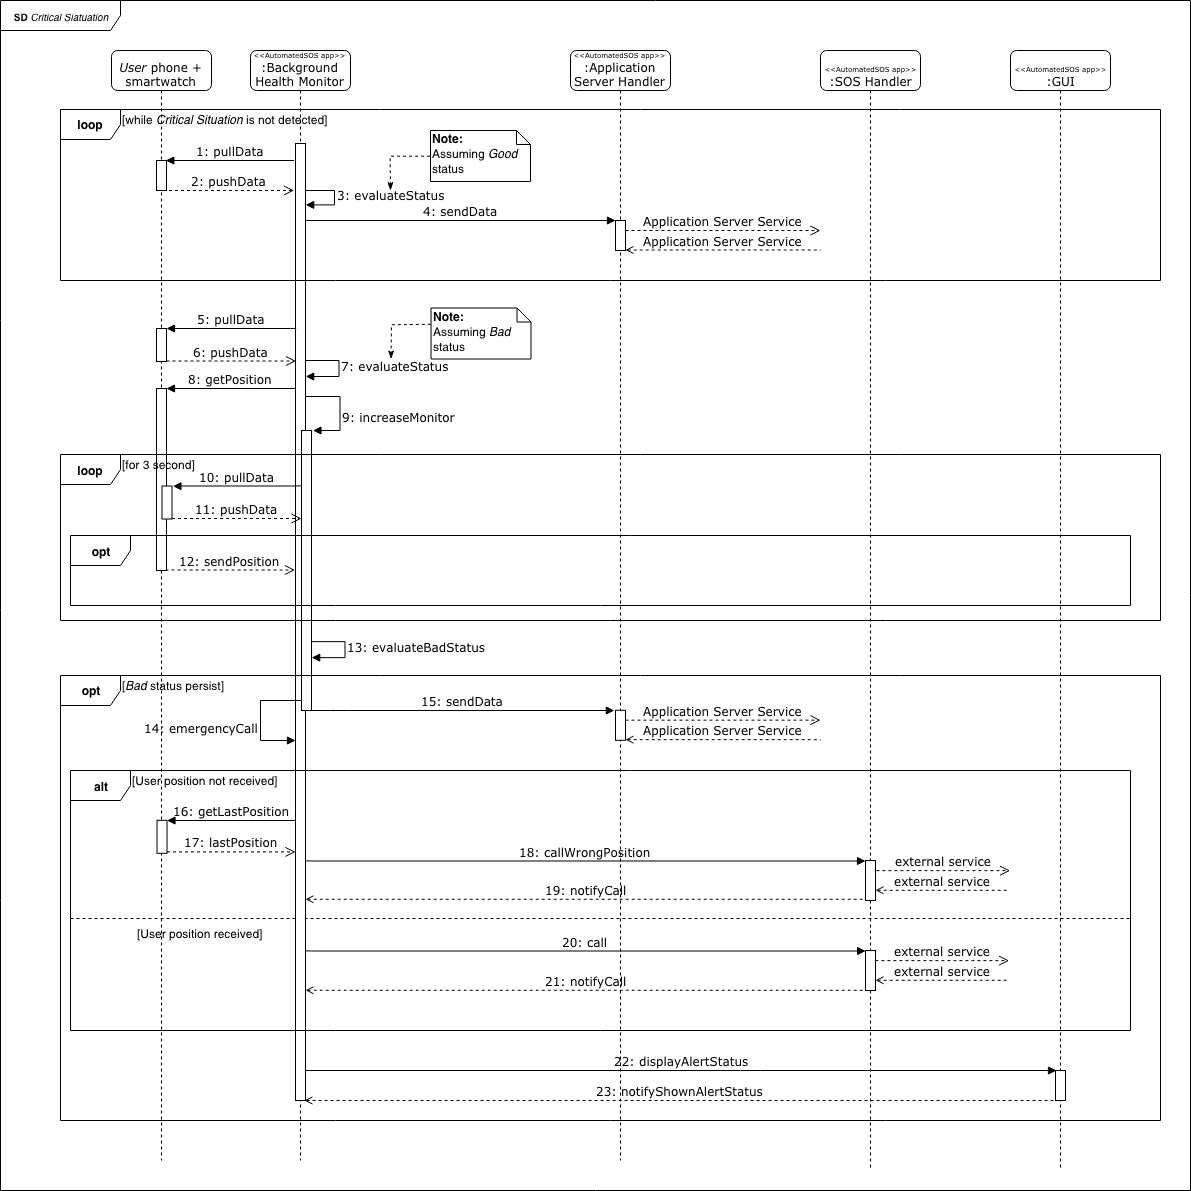
\includegraphics[width=\textwidth]{./img/sequence/criticalSituation.png}
    \hspace{0.05\linewidth}
    \centering
    \caption{\textit{Critical Situation} sequence diagram}
		\label{img:criticalSituation}
    \end{center}
\end{figure}

\begin{figure}[H]
  \begin{center}
  	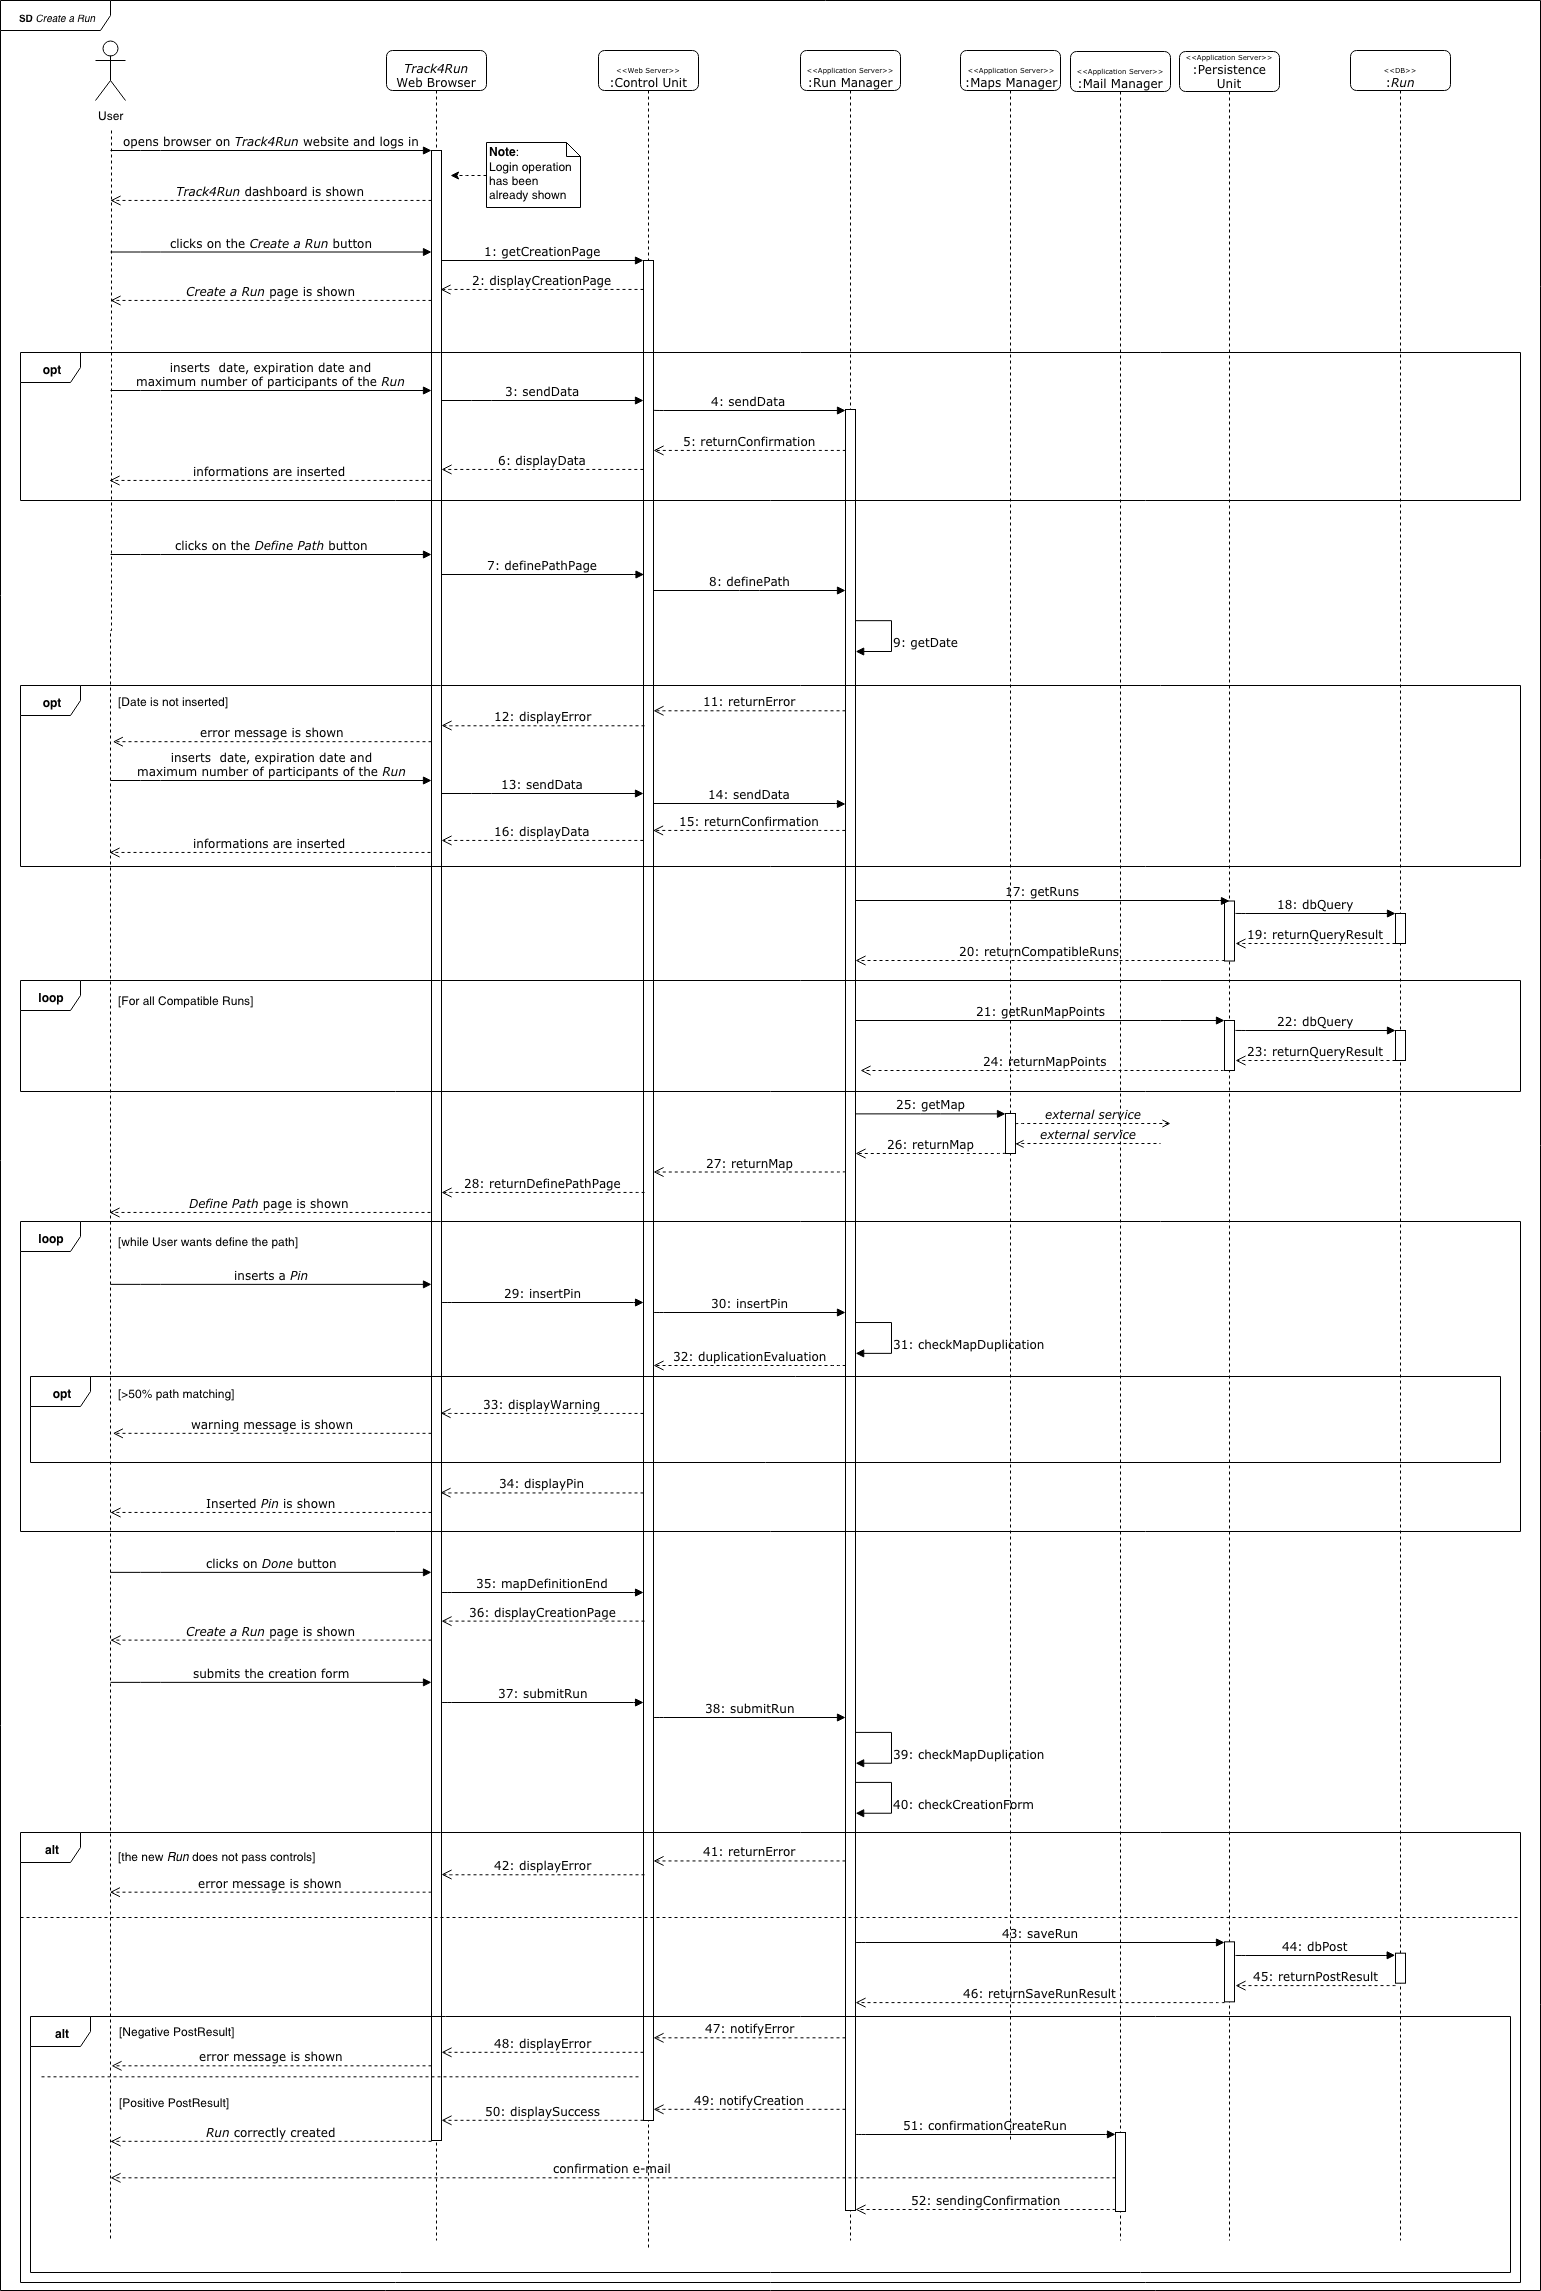
\includegraphics[width=\textwidth]{./img/sequence/createRun.png}
    \hspace{0.05\linewidth}
    \centering
    \caption{\textit{Create a Run} sequence diagram}
		\label{img:createRun}
    \end{center}
\end{figure}

\begin{figure}[H]
  \begin{center}
  	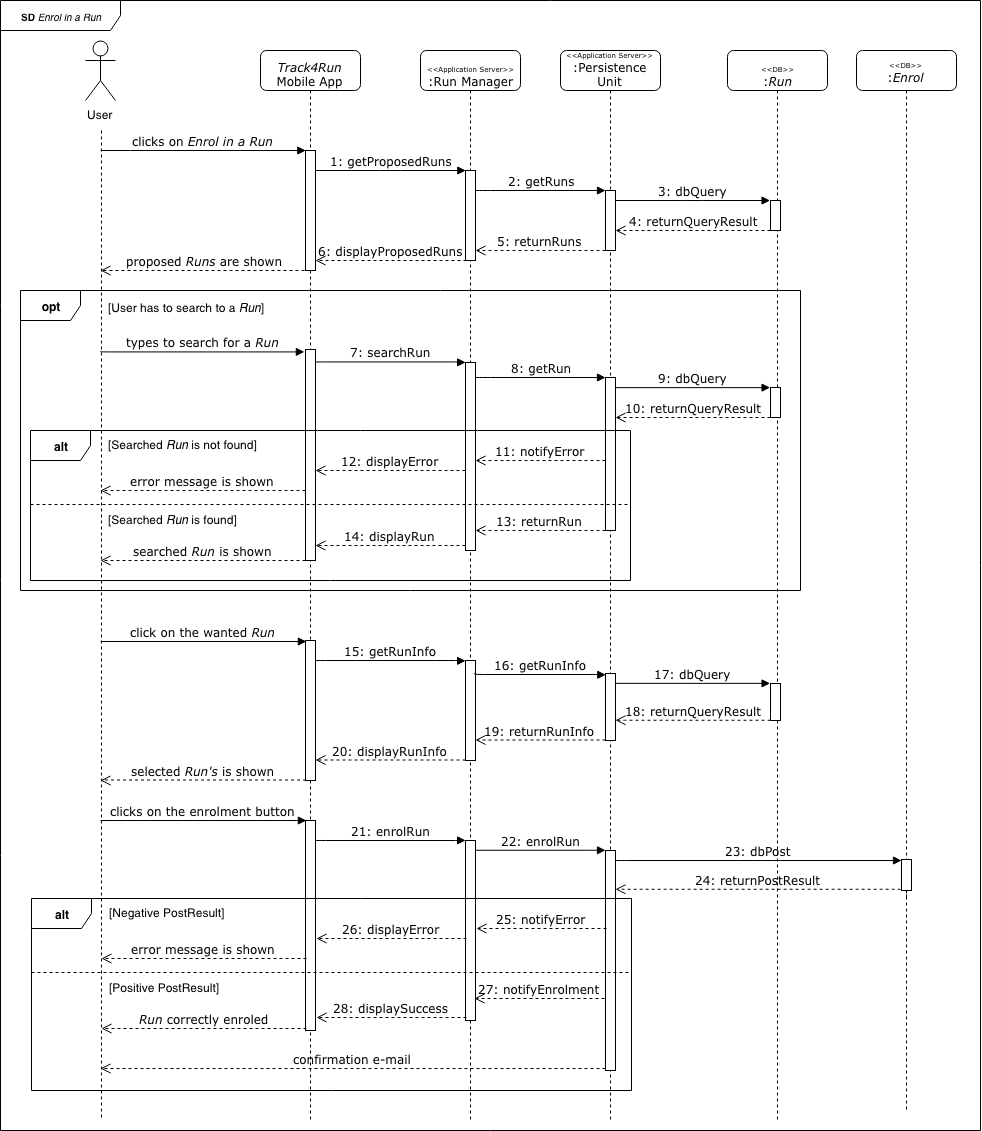
\includegraphics[width=\textwidth]{./img/sequence/enrolRun.png}
    \hspace{0.05\linewidth}
    \centering
    \caption{\textit{Enrol in a Run} sequence diagram}
		\label{img:enrolRun}
    \end{center}
\end{figure}

\begin{figure}[H]
  \begin{center}
  	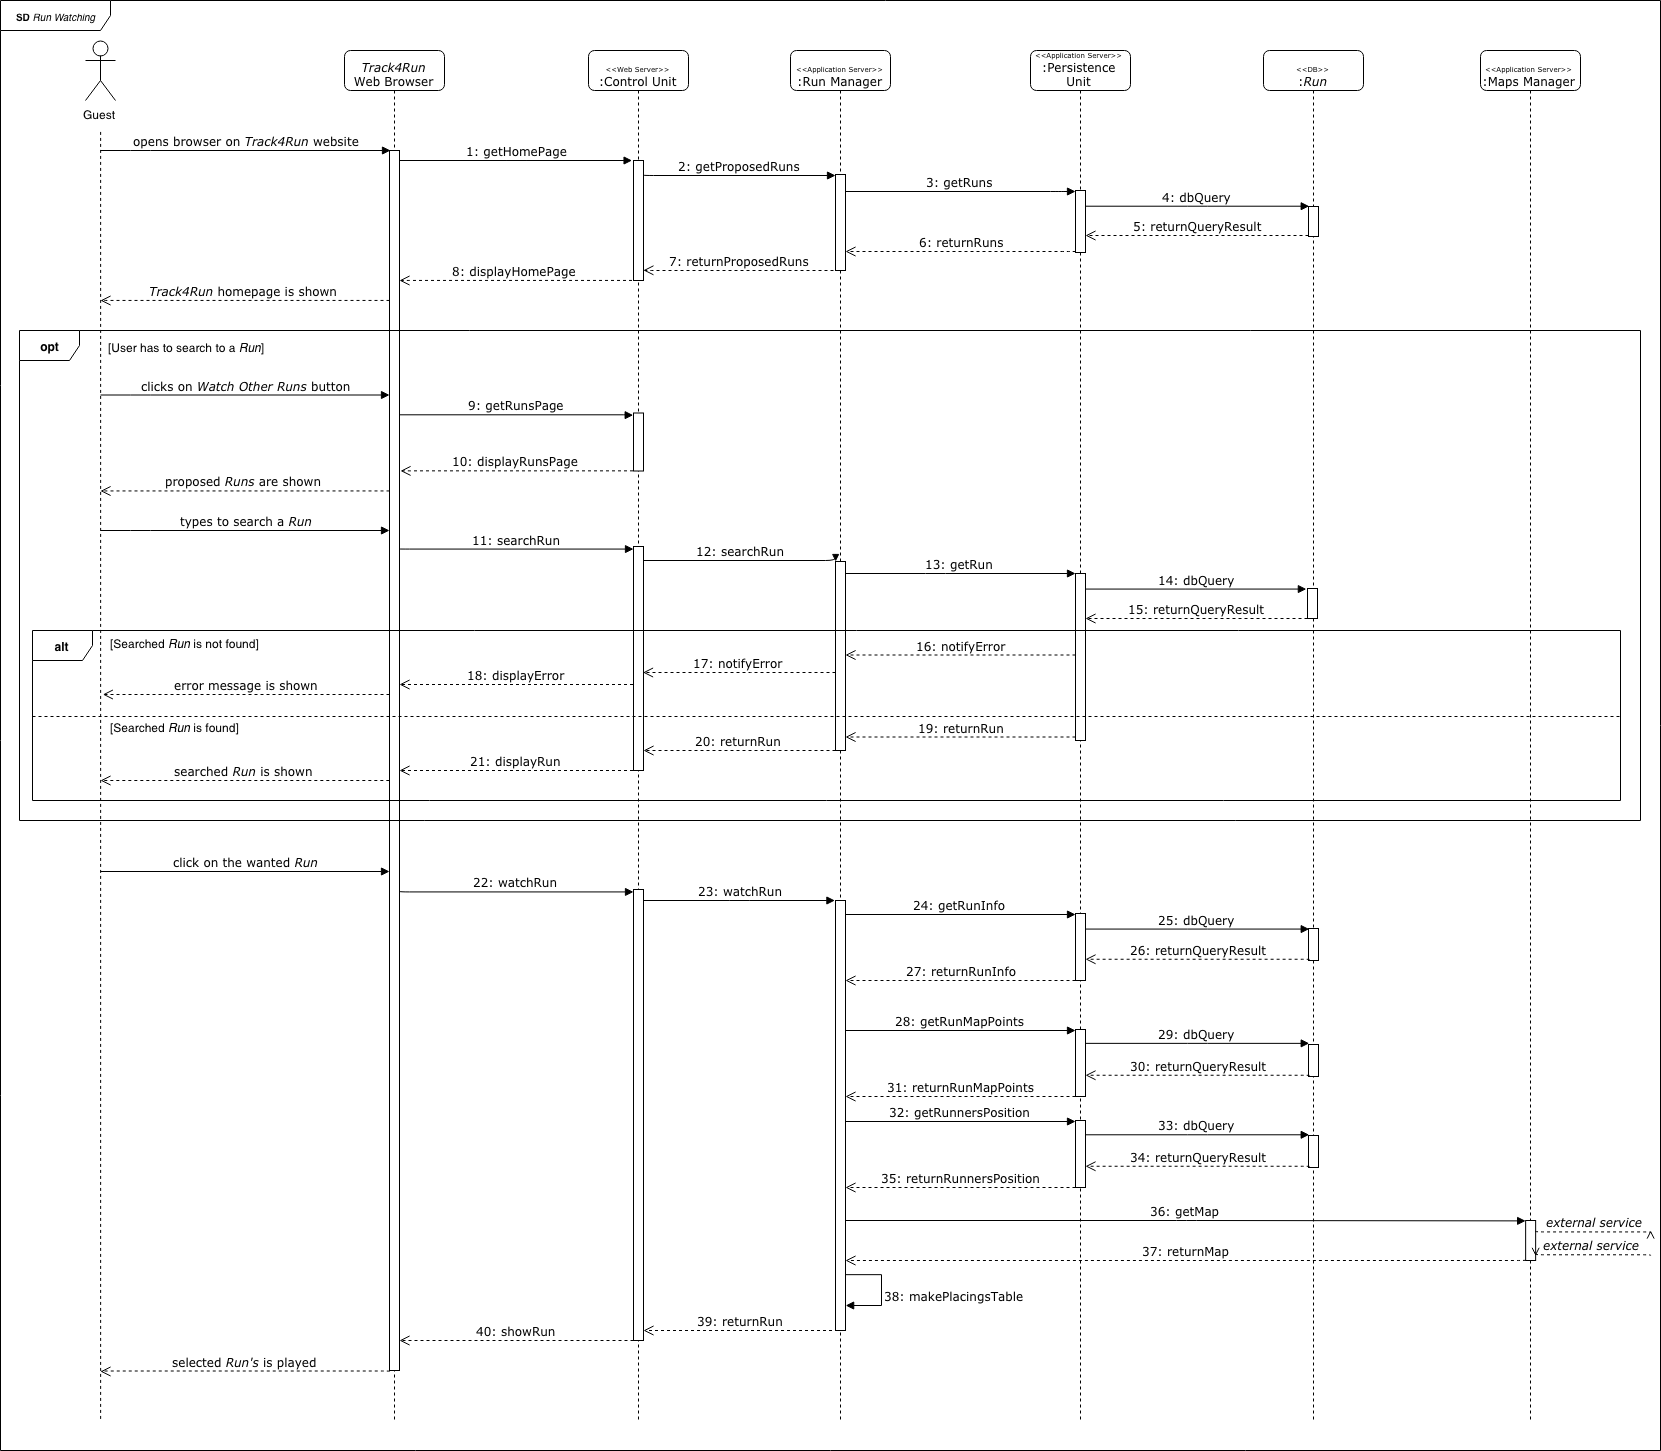
\includegraphics[width=\textwidth]{./img/sequence/watchRun.png}
    \hspace{0.05\linewidth}
    \centering
    \caption{\textit{Run Watching} sequence diagram}
		\label{img:watchRun}
    \end{center}
\end{figure}


\clearpage

\section{Component Interfaces}

\section{Selected Architectural Styles and Patterns}

\section{Other Design Decisions}
